\documentclass[12pt]{extarticle}
\usepackage[utf8]{inputenc}
\usepackage{graphicx}
\usepackage{url}
\usepackage{amsmath}
\usepackage{geometry}
\geometry{a4paper, top=2.5cm, left=2.5cm, right=2.5cm, bottom=2.5cm}

\title{\Huge \emph{Speech Recognition} \\ ELEC-E5510 \vspace{1cm} \\ Language recognition \vspace{1cm}}

\author{
Álvaro Orgaz Expósito \\ Student number: 802101 \\ \texttt{alvaro.orgazexposito@aalto.fi}
\and
Rachhek Shrestha \\ Student number: 802130 \\ \texttt{rachhek.shrestha@aalto.fi}
}

\date{\vspace{1cm} December, 2019}

\begin{document}

\maketitle

\begin{center} \vspace{\fill} 
\includegraphics[scale=1]{Figures/AaltoLogo.png} \vspace{5cm} \end{center}

\newpage

\tableofcontents

\newpage

\section{Introduction}

Language recognition is the automatic process to quantitatively determine which language is being spoken in a speech sample. In the last decades, several technological advancements in signal processing, pattern recognition, cognitive science and machine learning have allowed for incredible progress in this topic enabling applications such as spoken language translation or spoken document retrieval.\\

\noindent It is estimated that there exist several thousands of spoken languages in the world but the total number of phones required to represent all the sounds of these languages ranges only from 200 to 300 as explained by Haizhou et al. in \cite{Li2013SpokenLR}. Then, although there is a wide diversity in languages, many share similar characteristics like intonation, rhythm, stress pattern, phonetic system and phoneme sequences. Moreover, we know that humans recognize languages through a perceptual or psychoacoustic process that is inherent in the auditory system and, just like any other artificial intelligence technologies, spoken language recognition aims to replicate such human ability through computational means. Thus, the principal problem is how to scientifically measure the individuality of the diverse spoken languages in the world to classify correctly their speech samples.\\

\noindent Human listening experiments such as \cite{Li2013SpokenLR} suggest that there are different classes of language information or cues that contribute to the human perceptual process for spoken language recognition. Firstly, prelexical information including acoustic phonetics (physical sound patterns of the speech sounds as entities or phonemes that the human speech apparatus is capable of producing), phonotactics (constraints that determine permissible phones sequences or syllable structures in a language), and prosodic (features in running speech such as stress, duration, rhythm, and intonation). Secondly, lexical information of languages about their phonological system that governs how symbols are used to form words or morphemes, and their syntactic system that governs how words and morphemes are combined to form phrases. The lexical knowledge can be gained by experience and studies revealed that given only a little previous exposure humans listeners can effectively identify a language without much lexical information. Therefore, mainstream research about automatic language recognition systems uses acoustic phonetics and phonotactics information.\\

\noindent From a mathematical and engineering perspective the problem of language recognition starts from a speech waveform in an unknown language which is split into a sequence of frames with their respective acoustic feature vectors. Then, the problem is to assign the most likely language to this acoustic observation. But to deal with phones and phonotactic knowledge it is assumed that the speech waveform can be segmented into a sequence of phonemes which in practice is unknown and has to be decoded from the observation waveform with phone models.\\

\noindent In this project we are approaching the task by using state of the art artificial intelligence models, such as CNN and LSTM, as well as Fourier transforms to extract the Mel Spectrogram and MFCC features from labelled audio samples from 6 different languages. By using our classification approach, which is deeply explained in sections \ref{Data} and \ref{Methods}, we achieve an accuracy of 83\% in a test set. \textbf{Keywords:} automatic language recognition, signal processing, acoustic features extraction, machine learning, classifiers, CNN, LSTM.

\section{Literature study}

\noindent Language recognition has been well studied in the literature and there are several different approaches to build a language recognition system. During the whole project, we have read a large number of papers to acquire a better understanding of the past and current state-of-the-art approaches and solutions for this task. Here we provide an overview of the main previous approaches which we have used as reference and inspiration.\\

\noindent The paper \cite{Li2013SpokenLR} by Haizjou et al. has listed down a couple of recent advances. They report that the models used to build contemporary language recognition systems from labelled training data could be: 1) stochastic e.g. Gaussian Mixture Models (GMM) and Hidden Markov Model (HMM); 2) deterministic e.g. Vector Quantization (VQ), Support Vector Machine (SVM) and Neural Networks; 3) discrete stochastic e.g. N-gram Models. The paper also claims that acoustic-phonetic and phonotactic approaches are the most effective ones for modelling the characteristics of languages. There is also an introduction to advanced techniques that have explored the combination of different features and approaches to build the most state-of-the-art language recognition system which is composed of several subsystems that complement each other and are combined using an effective fusion technique.\\

\noindent There is another novel way of language identification developed in \cite{42540} and \cite{Tang:2018:PTN:3180719.3180730} which uses Long Short-Term Memory (LSTM) Recurrent Neural Networks (RNN). This technique effectively exploits temporal dependencies in acoustic data to learn relevant features for language discrimination. It is reported to achieve better performance than previously used Deep Neural Networks (DNN) based systems with a reduced number of parameters.\\

\noindent Finally, another important reference used to select a suitable model architecture and features maps extraction is \cite{inproceedings}. Indeed, for understanding and implementing well the concept of convolutional 1D layers we have used the article \cite{Conv1DKeras}.

\section{Data} \label{Data}

The dataset is a subset of approximately 50 hours of audio files from the Mozilla Common Voice speech dataset, freely available at \url{https://voice.mozilla.org}. This source provides a lot of hours of speech for many languages, but we have selected 6 (Estonian, German, Mandarin, English, Spanish, Farsi, and Kabyle) and a subset of samples for each one not shorter than 3 seconds. It is a very balanced dataset for the language recognition task of these 6 different languages. Moreover, the audio files have been converted from MP3 format to waveform WAV files at a frequency of 16 kHz with a normalized volume of -3 dBFS.\\

\noindent The dataset is split into speaker-disjoint train and test sets, which means that none of the test speakers has been used for training, in the following way:

\begin{itemize}
    \item German: In the training set 7053 files, total duration of 9 hours, and average file duration: 4.59 seconds. In the test set 494 files, total duration of 24.7 minutes, and fixed file duration 3 seconds.
    \item Spanish: In the training set 6527 files, total duration of 8.13 hours, and average file duration: 4.47 seconds. In the test set 452 files, total duration of 22.6 minutes, and fixed file duration 3 seconds.
    \item Estonian: In the training set 4818 files, total duration of 8.91 hours, and average file duration: 6.66 seconds. In the test set 487 files, total duration of 24.35 minutes, and fixed file duration 3 seconds.
    \item Farsi: In the training set 6337 files, total duration of 8.74 hours, and average file duration: 4.97 seconds. In the test set 516 files, total duration of 25.8 minutes, and fixed file duration 3 seconds.
    \item Kabyle: In training set 6676 files, total duration of 8.36 hours, and average file duration: 4.51 seconds. In the test set 486 files, total duration of 24.3 minutes, and fixed file duration 3 seconds.
    \item Mandarin: In the training set 4298 files, total duration of 8.03 hours, and average file duration: 6.71 seconds. In the test set 695 files, total duration of 34.75 minutes, and fixed file duration 3 seconds.
\end{itemize}

\noindent Note that all test audio files have exactly 3 seconds duration, which at a frequency of 16kHz corresponds to 48.000 audio samples. This fact determines the features preprocessing of the training audio files which have different durations.

\section{Methods} \label{Methods}

\subsection{Audio features extraction}

\noindent Firstly, we are going to introduce the acoustic features extraction used to prepare the inputs for the modelling method explained in section \ref{Modelling}. For each entire audio file (train and test sets with different durations) we have extracted:

\begin{itemize}
    \item[a)] Log-Mel-Spectrogram keeping 40 dimensions or filterbanks.
    \item[b)] Mel-Frequency Cepstral Coefficients (MFCC) keeping 40 dimensions.
\end{itemize}

\noindent This feature extraction has been implemented in Python using the module \textit{librosa}. The parameters configuration used is:

\begin{itemize}
    \item[-] Length of the FFT window (\textit{n\_fft}): 512 samples equivalent to 32ms.
    \item[-] Samples between successive frames (\textit{hop\_length}): 160 equivalent to 10 ms.
    \item[-] Sampling rate or frequency (\textit{fr}): 16 kHz.
    \item[-] Lowest/highest frequency (\textit{f\_min/f\_max}): 300/8000 Hz.
\end{itemize}

\noindent Note that for test audio files with a fixed duration of 3 seconds, the shape of the feature is exactly (297,40) where 297 is the number of frames equal to $1+(48000-512)//160$ and 40 the kept dimensions.

\begin{figure}[h]
\centering
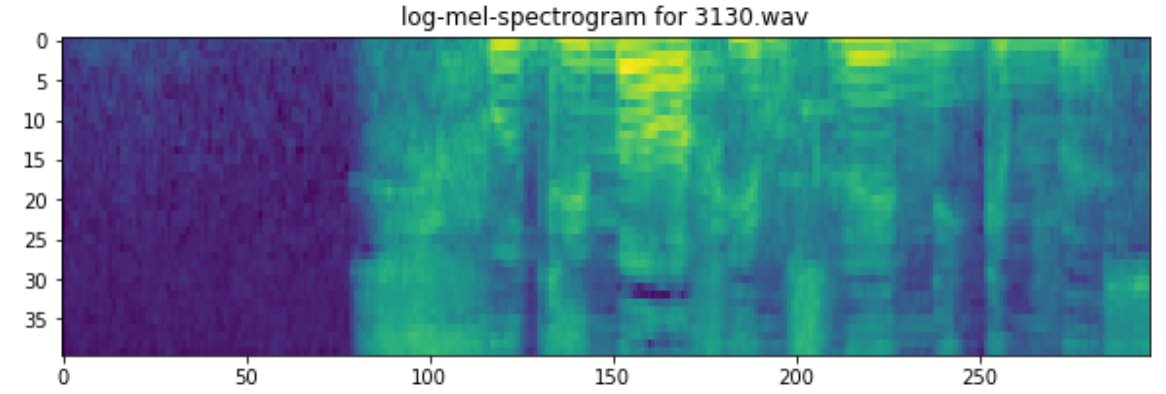
\includegraphics[width=\linewidth]{Figures/1.png}
\caption{Feature extraction Log-Mel-Spectrogram for a test audio example. Statistics: shape (297,40), min -13.3, max 4.1, mean -4.1, std 2.5.}
\label{fig1}
\vspace{1cm}
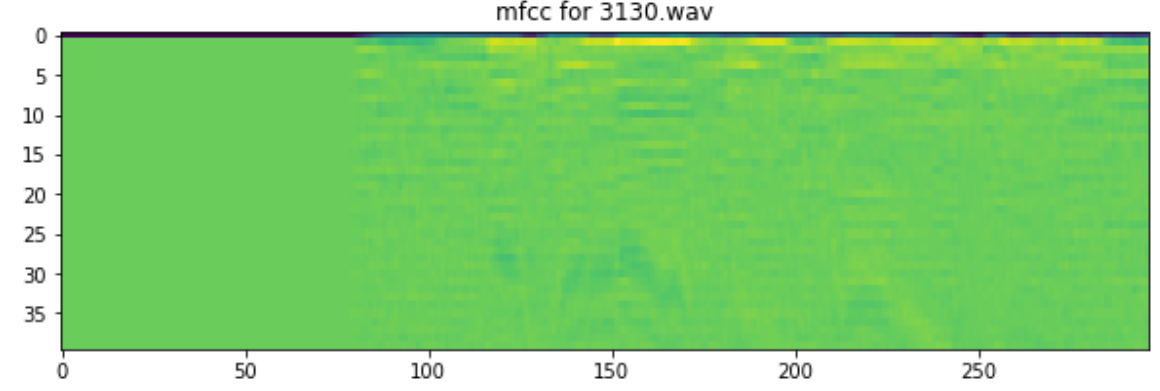
\includegraphics[width=\linewidth]{Figures/2.png}
\caption{Feature extraction MFCC for a test audio example. Statistics: shape (297,40), min -648.6, max 191, mean -8.9, std 78.6.}
\label{fig2}
\end{figure}

\subsection{Features preprocessing}

Secondly, we are going to introduce the preprocessing applied to the extracted features before feeding the model. Since we are testing audio files of precisely 3 seconds, it is fair that each input feature sample has the same shape as the test ones. Then, we have split the features extracted from the training data audio files into equal chunks of shape (297,40) by using moving windows of hop length 100 frames. It is equivalent to $100*160=16.000$ samples or 1 second. Note that we delete the remaining seconds after the last possible complete chunk. The lower the number of frames between chunks, the lower the duration dropped, and more new chunks or training samples generated.\\

\noindent The reasoning behind this is:

\begin{itemize}
    \item[-] consider the time context of each original audio file without splitting the files exactly every 3 seconds,
    \item[-] data augmentation since we are creating from 35k training audio files around 95k training samples versus 47k samples by splitting exactly every 3 seconds,
    \item[-] and do not discard many remaining seconds or frames after the last possible split.
\end{itemize}

\subsection{Modelling} \label{Modelling}

\noindent Thirdly, we will introduce the 2 modelling techniques that we have used for this classification task.\\

\noindent \textbf{CNN}\\

\noindent The first one is a Convolutional Neural Network (CNN). Since CNNs are very popular models we are going to go deeper only about the type of convolutional filters used which is convolutional 1D filters. As explained in \cite{Conv1DKeras}, CNNs work the same way whether they have 1, 2, or 3 input dimensions, however, the difference is the structure of the input data and how the filter, also known as a convolution kernel or feature detector, moves across the data. In our case, a features sample is made up of 297 frames and each one is a 40-dimensional vector that represents it. The filter covers at least one frame, and kernel size parameter specifies how many frames the filter should consider at once. In Figure \ref{fig3} we can see how the filter scans the data. On the other hand, 2D convolutional filters move over the input features both horizontally and vertically.

\begin{figure}[h]
\centering
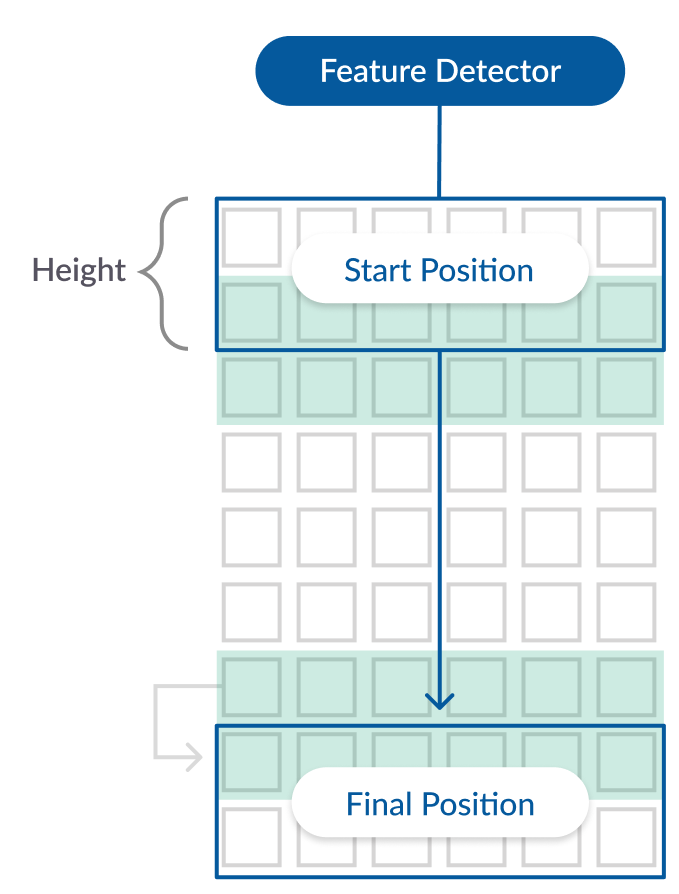
\includegraphics[width=5cm]{Figures/3.png}
\caption{Convolutional 1D filters.}
\label{fig3}
\end{figure}

\noindent About the CNN model architecture, in Figure \ref{fig4} you can see all the convolutional 1D layers used with \textit{ReLU} activation function, respective strides (1,2,1,1) and kernel size (6,7,1,1), as well as the global average pooling layer followed by fully connected layers and a final \textit{softmax} activation function for the 6 output nodes.\\

\begin{figure}[h]
\centering
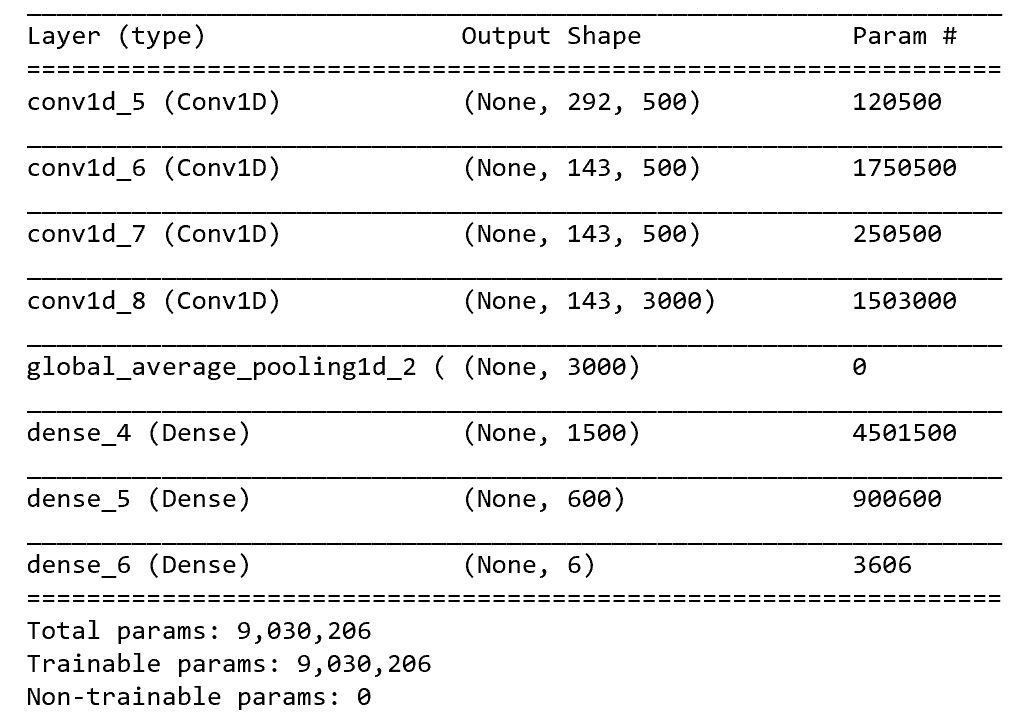
\includegraphics[width=10cm]{Figures/4.png}
\caption{CNN model architecture.}
\label{fig4}
\end{figure}

\noindent \textbf{LSTM}\\

\noindent Secondly, we have implemented a LSTM model. LSTM Neural Networks have an edge over the conventional feed-forward network and Recurrent Neural Networks (RNN). This model can selectively ``remember" and ``forget" patterns for a longer duration of time than basic RNN. Their basic architecture is composed of \textit{forget gates} responsible for removing information from cell states, \textit{input gates} that add information to cell state, and \textit{output gates} that select useful information as output. About the LSTM model architecture, in Figure \ref{fig5} you can see the LSTM layer with 32 units followed by a fully connected layer and a final \textit{softmax} activation function for the 6 output nodes.

\begin{figure}[h]
\centering
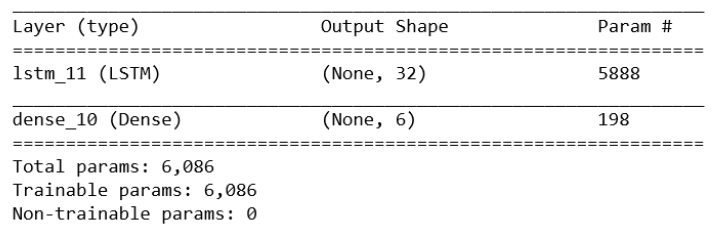
\includegraphics[width=10cm]{Figures/10.png}
\caption{LSTM model architecture.}
\label{fig5}
\end{figure}

\subsection{Training procedure}

According to the training method used, it is important to explain how we tackle the problem of working with 52 hours of audio files to train the models. We have implemented this project using Python and the module \textit{Keras} of \textit{Tensorflow}. Since the preprocessed features occupied up to 15GB depending on the experiment, we used the \textit{fit\_generator Keras} function to iteratively load a batch of size 40 samples. Each batch contained samples from all languages to balance the training and for completing each epoch including all training samples. About the loss function, we have used \textit{Categorical Cross Entropy} because this is a multiclass classification problem. We have optimized it by using \textit{Adam Amsgrad} because it is an adaptive learning rate optimization algorithm that’s been designed specifically for training deep neural networks \cite{AdamOptimizer}. And the learning rate is 0.001. Moreover, early stopping in train and test sets for accuracy and loss metrics have been used in all the experiments.

\section{Experiments}

The main objective has been to build an end-to-end acoustic classifier (using only language labels and audio files) and for doing that, we have developed different modelling experiments to find the optimal performance.\\

\newpage

\noindent \textbf{CNN}\\

\noindent \underline{Experiment 1:} The first experiment compares the performance of the designed CNN model with different input features: Log-Mel-Spectrogram with 40 dimensions kept, Log-Mel-Spectrogram with 80 dimensions kept, Log-Mel-Spectrogram with 40 dimensions kept without moving window when creating multiple chunks of 3 seconds, and MFCC with 40 dimensions kept.\\

\noindent \underline{Experiment 2:} The second experiment compares the best result of experiment 1 with the same case but normalizing the input features by frames.\\

\noindent \underline{Experiment 3:} The third experiment compares the best result of experiment 2 with the same case but adding a \textit{Dropout} layer and \textit{Ridge} regularization.\\

\noindent \underline{Experiment 4:} The fourth experiment compares the best result of experiment 3 with the same case but modifying the speed of the input audios to 0.9x. It is a method of slowing down the audio files which at the same frequency level will give as more frames in the input features so it is working as data augmentation too.\\

\noindent \textbf{LSTM}\\

\noindent \underline{Experiment 5:} The fifth experiment compares the performance of the designed LSTM trained with the same features normalized MFCC with 40 dimensions. It is compared with a different number of units: 32, 100 and 200.

\section{Results}

In Figure\ref{fig6} we can find the result of experiment 1. We can observe that MFCC and Log-Mel-Spectrogram with 80 dimensions are not providing good results. Probably we would need to normalize those features since their variance is higher. Moreover, using moving windows when splitting the training features as explained before does not seem to increase performance but it helps to converge faster (remember that we are using early stoppings), so we will continue with this model.

\begin{figure}[h]
\centering
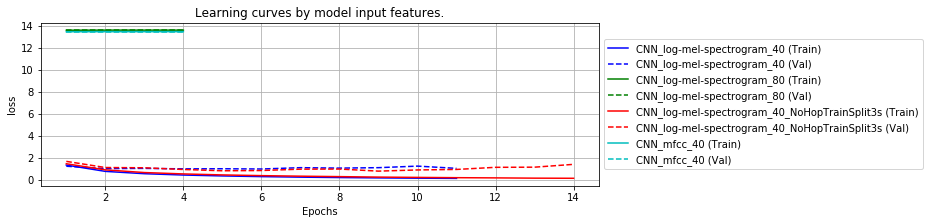
\includegraphics[width=\linewidth]{Figures/5.png}
\caption{Loss curves of experiment 1. Respective accuracy curves in appendix.}
\label{fig6}
\end{figure}

\newpage

\noindent In Figure \ref{fig7} we can find the result of experiment 2. Clearly, the features normalization is boosting the performance so we will continue with this model.
\begin{figure}[h]
\centering
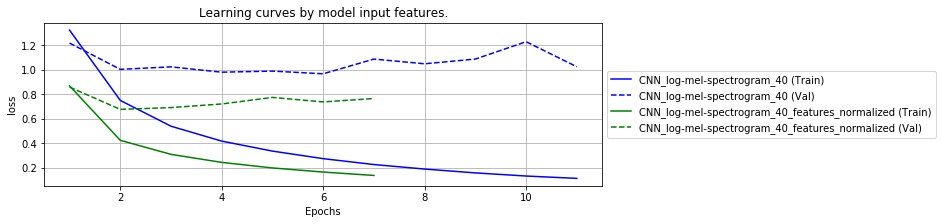
\includegraphics[width=\linewidth]{Figures/6.png}
\caption{Loss curves of experiment 2. Respective accuracy curves in appendix.}
\label{fig7}
\end{figure}

\noindent In Figure \ref{fig8} we can find the result of experiment 3. Clearly, the regularization components are increasing the training loss but reducing the validation loss so we will continue with this model.
\begin{figure}[h]
\centering
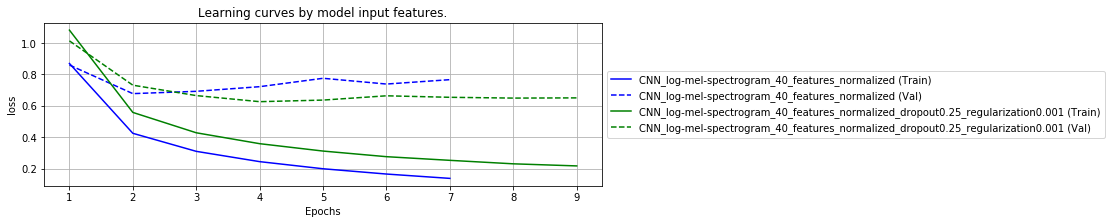
\includegraphics[width=\linewidth]{Figures/7.png}
\caption{Loss curves of experiment 3. Respective accuracy curves in appendix.}
\label{fig8}
\end{figure}

\noindent In Figure \ref{fig9} we can find the result of experiment 4. As we can observe, we do not find improvements by slowing down the speed.

\begin{figure}[h]
\centering
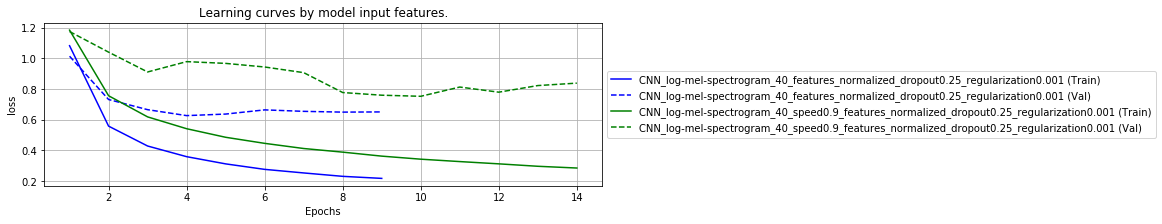
\includegraphics[width=\linewidth]{Figures/8.png}
\caption{Loss curves of experiment 4. Respective accuracy curves in appendix.}
\label{fig9}
\end{figure}

\noindent In Figure \ref{fig10} we can find the result of experiment 5. Clearly, increasing the number of LSTM units from 32 to 100 boosts the performance but increasing up to 200 not. LSTM with 100 and 200 follow a similar training curve. So we select 100 units as the best LSTM model. Increasing the LSTM units also increased the time required to train the model. 

\begin{figure}[h]
\centering
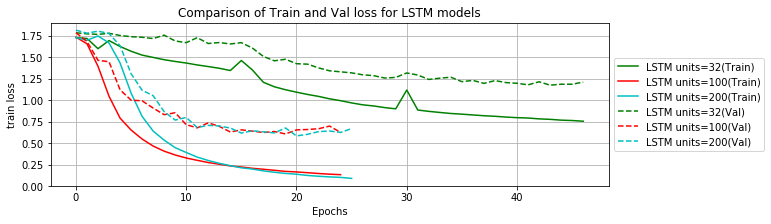
\includegraphics[width=\linewidth]{Figures/11.png}
\caption{Loss curves of experiment 5. Respective accuracy curves in appendix.}
\label{fig10}
\end{figure}

\newpage

\section{Conclusions / Discussion}

Firstly, according to the CNN experiments, we have seen that increasing the number of kept dimensions in the Log-Mel-Spectrogram does not improve the results as well as using MFCC features. On the other hand, the design of the preprocessing technique using hop splits like moving windows to get the same test features shape boosts the performance a bit. Moreover, adding a \textit{Dropout} layer plus \textit{Ridge} regularization reduce the overfitting of the model enabling higher test accuracy up to 81\%. Finally, speeding down the input audio files does not improve our results.\\

\noindent Secondly, according to the LSTM experiments, a comparatively simpler model architecture than CNN gives decent accuracy results. A larger model learns faster but might overfit quickly. In short, LSTM has proved to be a very effective model in our experiments, although it takes a long time to train.\\

\noindent Overall, both CNN and LSTM were able to give similar accuracy but LSTM had simpler model architecture, hence less number of total trainable parameters. About the most difficult language to predict, we can see from Figures \ref{fig10} and \ref{fig11}, which contain the confusion matrix for the best CNN and LSTM models, that Farsi is relatively the hardest language to recognize with an accuracy around 65\% and Mandarin is way easier achieving an accuracy higher than 90\%.

\begin{figure}[h]
\centering
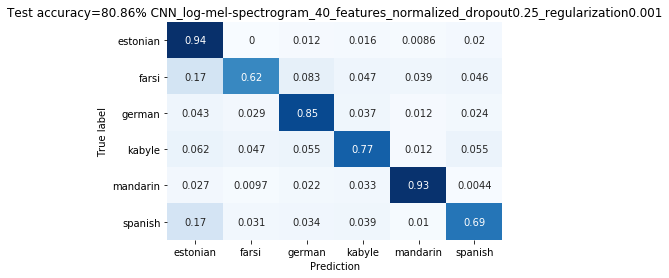
\includegraphics[width=12cm]{Figures/9.png}
\caption{Confusion matrix of best CNN model in test set.}
\label{fig11}
\end{figure}

\begin{figure}[h]
\centering
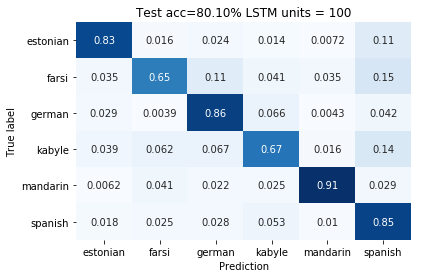
\includegraphics[width=7.5cm]{Figures/12.png}
\caption{Confusion matrix of best LSTM model in test set.}
\label{fig11}
\end{figure}

\section{Division of labor}

Álvaro contributed to the literature study, development of project plan, report documentation, most part of the data preprocessing, and modelling all the experiments related to CNN. Similarly, Rachhek contributed to the literature study, report, partly with the preprocessing needed for LSTM experiments, and modelling all LSTM experiments. Both members jointly presented the findings of the project in the class on December 11 2019.

\section{Acknowledgements}

We would like to thank our lecturer and professor Mikko Kurimo for giving us the opportunity to work on this project. We are also really grateful to Matias Lindgren who guided us and patiently answered our questions every step of the way.

\newpage

\addcontentsline{toc}{section}{References}
\bibliographystyle{ieeetr}
\bibliography{bibliography.bib}

\newpage

\addcontentsline{toc}{section}{Appendix}
\section*{Appendix}

\subsection*{Code}

Please, find the code in the GitHub repository \url{www.github.com/alvarorgaz/Language-} \url{Speech-Recognition-with-CNN}.

\subsection*{Rest of figures}

\begin{figure}[h]
\centering
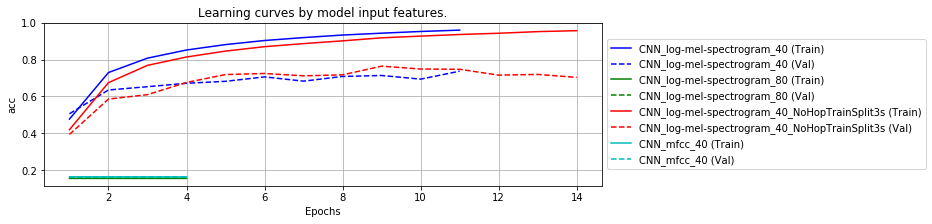
\includegraphics[width=\linewidth]{{Figures/5.2}.png}
\caption{Accuracy curves of experiment 1.}
\vspace{0.4cm}
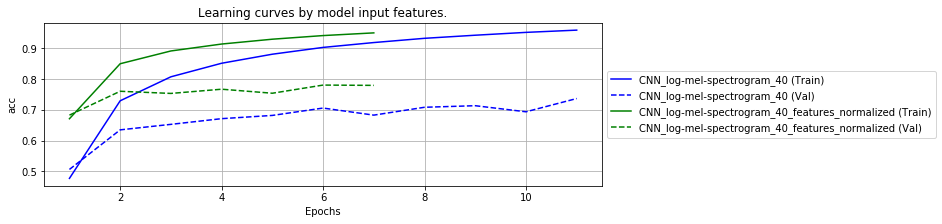
\includegraphics[width=\linewidth]{{Figures/6.2}.png}
\caption{Accuracy curves of experiment 2.}
\vspace{0.4cm}
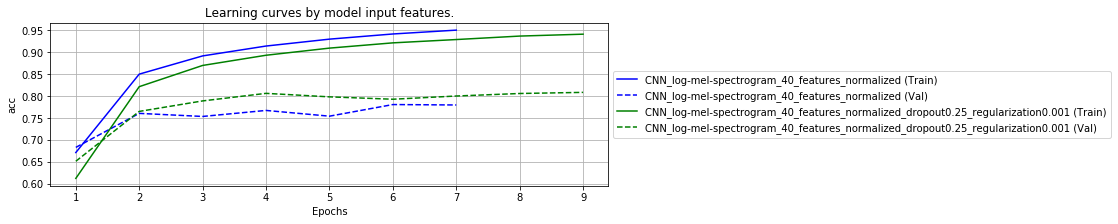
\includegraphics[width=\linewidth]{{Figures/7.2}.png}
\caption{Accuracy curves of experiment 3.}
\vspace{0.4cm}
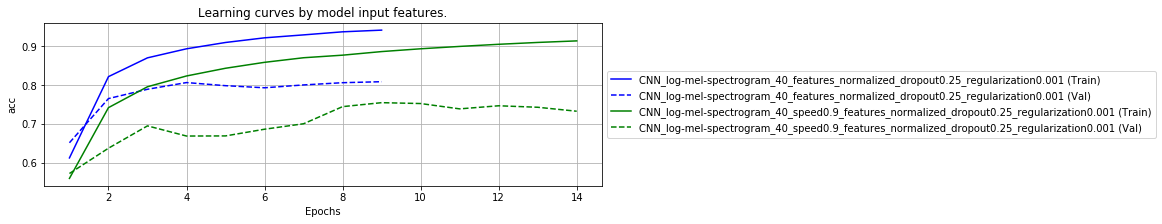
\includegraphics[width=\linewidth]{{Figures/8.2}.png}
\caption{Accuracy curves of experiment 4.}
\end{figure}

\newpage

\begin{figure}[h]
\centering
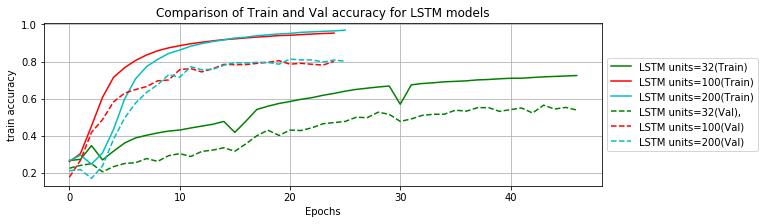
\includegraphics[width=\linewidth]{{Figures/11.2}.png}
\caption{Accuracy curves of experiment 5.}
\end{figure}

\vspace{\fill}

\end{document}